\chapter{Analýza}
Súčasťou tejto kapitoly je zdôvodnenie jednotlivých rozhodnutí, ktoré sme navrhli. Chceme vytvoriť taký virtuálny svet, v ktorom môzeme pozorovať chovanie robotov, ktorý obsahuje rôzne objekty a v ktorom je netriviálne napísať dobrý program.
\section{Virtuálny svet}
Neoddeliteľnou súčasťou hry je virtuálny svet (prostredie), v ktorom sa bude súboj odohrávať. Najskôr vysvetlíme, čo všetko svet obsahuje, ako sa v ňom žije z hľadiska robota, na čo musí dbať uživateľ ( ako sa narába s objektom v programe) a ako jednotlivé pravidlá prispievajú k úspešnosti algoritmu. \\ 
% máme dvojrozmerny svet
Uvažovaný svet bol vybraný dvojrozmerný, pretože poskytuje dostatok možností pre dianie na ploche (smer pohybu, zrozumiteľne vykresľovanie stavu, podpora fyzikálnych zákonov a pod.) a súčasne nie je obtiažne implementovateľný. Tým sme sa vyhli obom predstaveným extrémom, a to 1D a 3D prostrediu.
\subsection{Súčasti virtuálneho sveta} %tu by sme mali vediet, ze robotovo telo je to hlavne -> uvedene pod sekciou
\label{staticky svet}
Základnou súčasťou virtuálneho sveta sú roboti, ktorí sa smú pohybovať. Bez ďaľších objektov by bolo logickým vyústením hry len jednoduché nájdenie robota.
Roboti sa môžu brániť iba pohybom (nič iné by vo svete nebolo). Tento prístup je zaujímavý, ale jednotvárny, ráta sa stále s tým istým stavom sveta). Preto uvažujeme aj o ďaľších objektoch. \\%slo by
\indent Hráč aktívne nevstupuje do vykonávania algoritmu, preto je nutné charakterizovať virtuálny svet z hľadiska robota, resp. uživateľovou znalosťou objektov, na ktoré môže robot reagovať.\\
\\
\indent Objekty uvažované vo svete vzhľadom na to, čo môže algoritmus využívať, sú nasledovné:
\begin{description}
\item[Robot ako objekt]\hfill \newline %vlastnosti robotov, preco by ali byt modifikovane, kontrola, ci to ma byt ako prve
%tu chcem napisat, ze robot sam je objekt, kedze reaguje a ostatnych robotov
Základnou schopnosťou robota je, že môže ubližovať ostatným robotom. Povedali sme, že robot získava informácie o objektoch svojho sveta, teda roboti sami musia mať vlastnosti objektu sveta. Tym sme sa úspešne vyhli konceptu ARES-a, ktorý nedokáže zistiť objekty k nemu nepatriace.
\newline
%Rozsirit, preco je tento sposob dobry, ako inak sa da ublizovat
%to co neni na koniec? Alebo pomiesane?
\item[Strely] \hfill %musia tam byt strely kvoli vypocitaniu utoku 
\newline % tu sme stale bez stien
%MOMENT, ci to nahodou nie je dynamika?
Roboti by mali vedieť útočit na diaľku. To možno docieliť viacerými spôsobmi:
\begin{itemize}
\item Robot zaútočí z diaľky na konkrétne miesto okamžite je známy výsledok útoku. To dáva užívateľovi jasnú spätnú väzbu. V okamihu útoku na diaľku je treba rozhodnúť, kedy smie robot zaútočiť týmto spôsobom. Ak môže robot zaútočiť na akékoľvek miesto, potom ostatní roboti nielenže nemajú možnosť sa útoku vyhnúť, ale strácaju aj informácie o tom, odkiaľ útok prišiel (na každé políčko môže byť zaútočené). Stratégie sa zredukujú na dva príncípy - náhodne útočenie z diaľky na nejaké miesta alebo na pohyb robota dovtedy, pokiaľ sa nenájde cieľ a následne na masívny útok na cieľ. Pripomína to hru typu lode, ktorá neponúka dostatočný priestor pre vymýšľanie stratégií. \\ %skontrolovat, ci neexistuje ieco fikanejsie
\item Minimálne je teda nutné obmedziť pravidlami, na ktoré miesta sa môže útočiť z diaľky. Intuitívne a ľahko zobraziteľné je vymedziť polomer zásahu, robot bude môcť útočiť len do určitej vzdialenosti. Stále je ale nemožné spozorovať útok na diaľku a tak sa mu vyhnúť.  Od predchádzajúcej metódy je však minimálne zaistená väčsia možnosť taktického manévrovania. Robot si z útoku bude vediet približne odhadnúť, že niekde v okolí je nepriateľský robot. V ARES-e toto nie je možné, aj keď útok na hocijaké políčko áno.
\item Ďaľšou možnosťou je vytvorenie strely. Strela je objekt, ktorého jedinou činnosťou je pohybovať sa predvídateľne vpred po dobu dopredu známeho času  (v danom smere výstrelu). Dodatočne pridávame, že strela skončí svoju činnosť aj v okamihu, keď spraví útok na blízko - zasiahne robota. V tom okamihu bude robot informovaný o úspechu tým, že strela vybuchne a robot sa súčasne sa nemusí obávať toho, že strela aj jeho neskôr zasiahne. To je vlastne robotova odmena. %napriek tomu, že algoritmus dosiahol čiastočný úspech. 
Pre boj z diaľky bol teda vytvorený nový objekt - strela.
\end{itemize}
Robot útočí tým, že na cieľ vystrelí, strela následne spraví útok na blízko. Tento prístup poskytuje väčšiu voľnosť pri útočení, nakoľko stači rozhodnúť, v ktorom smere má strela ísť. Takto je možné približne odhadnúť smer, odkiaľ strela prišla. To je dôležité pri rozhodovaní sa, či robota napadnúť priamo (nablízko), alebo odpovedať streľbou. \\
\indent Robot nebude mat nekonečnú možnosť strieľať, inak by hra nekládla nároky na zistenie, ktorým smerom je vhodné zaútočiť. Navyše ak robot strieľa neobmedzene, potom môže byt hracie pole zahltené strelami, čo výrazne spomalí simuláciu. Preto je počet striel obmedzený. Strelivo ale nie je možné dopĺňať. Preto sa strela okamžite po vykonaní útoku vráti k robotovi, ktorý ju vystrelil a ten ju môže použit znova. Takto robot okamžite zistí úspešný zásah.%<< zujimavy napad
%To, ze steny poskytuju ukryt pre robota tiez znamena, ze steny obmedzuju vyhlad robota.
%Este nejaky sposob planovania utoku na dialku?
\item[Steny] \hfill \newline
\indent Ďaľším uvažovaným prvkom sú objekty, ktoré môže robot využívať na svoju obranu. Útočiť na robota môžu objekty len z blízka ( robot z blízka alebo z diaľky, čo je ale vlastne strela z blízka).  Vo virtuálnom svete potom potrebujeme niečo, čo obmedzí pohyb. Týmito objektami budú steny. Robot ich môže využívat ako strategický úkryt, podobne ako vojaci využívaju terénne nezrovnalosti. %zase pogamut %TOTO BY SOM DAL PREC CELE? Ja chcem povedat, ze tam robot za to nebude viodet! Ukryt je definovany tak ze ho nezasiahne strela, anie nie, ze nebude visietVzhladom na to, ze steny budu zabranovat pohybu, mali by zabranovat aj robotovi vidiet objekt za stenou. Tato informacia by totiz znevyhodnila robota, ktory sa sikovne skryl. <tot jest blbost, mmnt, spatne argumentujem>
\newline
\item[Prepadliska - zakázané miesta] \hfill \newline
\indent Zaujímavým strategickým obmedzením sú miesta, na ktoré robot za žiadnych okolnosti nesmie stúpiť. V prípade POGAMUT-u sú to priepasti, jamy, tekutá láva a pod. V ARES-e zase miesto v pamäti, ktoré obsahuje neplatnú inštrukciu. Existencia prepadlísk umožňuje plánovať stratégiu využívajúcu silný útok z diaľky a vyhne sa silným útokom zblízka. 
\newline
\item[Štartovné pozície robota]\hfill
\newline
Ak roboti nemajú dopredu dané miesto na mape, potom sa ich štartovné pozície musia generovať buď náhodne alebo vypočítať tak, aby umiestnenie bolo nejakým spôsobom spravodlivé (nebol zvýhodnený ani jeden robot ). Rozoberme si podrobnejšie jednotlivé ne/výhody virtuálneho sveta bez štartovných pozícií robotov:
%problem zistovania vhodneho miesta
%roboti vedla seba, vyhody, nevyhody? - ani jedno. neskor sa to mohla stat,treba tym ratat
%nevyhoda, ze dopredu neviem
\begin{description}
\item[Roboti vygenerovaní vedľa seba] \hfill \newline
Táto situácia môže nastať kedykoľvek počas behu programu, robot na ňu musí vedieť zareagovať. Preto jenáhdné generovanie vlastne spravodlivé.
\item[Roboti rovnomerne rozhádzaní po svete] \hfill \newline To môže zabrať netriviálne veľa času, obzvlášť ak je virtuálneho sveta zložená z veľkeho množstva stien a úzkeho priestoru pre pohyb robotov. %diskutabilne
\end{description}
\indent Kvôli zabezpečeniu spravodlivosti generovania pozícií robotov bude použitá heuristika. No je otázne čo chápať pod spravodlivosťou. Robot má za úlohu reagovať na každú situáciu, nie je preto nutné uvažovať o špeciálne vypočitaných miestach a tak pojem spravodlivosť stráca svoj význam.\\
Problémom zostáva množstvo robotov na mape a dlhé generovanie počiatočných pozícií. Z tohoto dôvodu sa pristúpilo k možnosti vytvorenia štartovacích políčok. To prináša okrem iného aj možnosť definovať, pre maximálne koľko robotov je mapa ideálna (ráta sa s týmto maximálnym počtom robotov). Ak ale uživateľ zadá viac robotov, simulácia sa aj potom môze uskutočniť. Je nutné len uživateľa upozorniť, že prebehol pokus umiestniť robota náhodne a či bol tento pokus úspešný. Teraz si už ale môžeme dovoliť dopredu daný počet pokusov a nepokúšať sa tak zbyttočne dlho. Po neúspechu nasleduje odstránenie robota zo simulácie. Ak aj pokus nebol úspešný, nič významné sa nedeje, pretože existuje na mape virtuálneho sveta dostatočné množstvo robotov, umiestnených na štartovacích políčkach.
\end{description}

\subsection{Život v prostredí} %mame ublizovanie +vlastnosti robotov
Roboti žijú vo svete a snažia sa zničiť ostatných. Nato vplývajú nasledovné vlastnosti robotov. \\
\begin{itemize}
\item Jednou z nich je {\bf veľkosť útoku}. To je vyjadrené celým číslom. Tak sa dá škoda zistiť presne a neobjavia sa problémy s malými číslami alebo zlomkami, ako je to v prípade reálnych čísel ( v C je napríklad 0 vyjadrená ako malé nenulové číslo). Čim väčšie číslo, tým väčšia škoda sa deje robotovi. 
\item V prípade vzdialeného útoku je tiež dôležitou otázkou, {\bf ako ďaleko } môže robot zaútočiť. Ak je toto čislo vopred dané, mal by o tom robot vedieť dopredu, aby mohol svoj algoritmus prispôsobit.
\item Útok robotov prebieha na úrovni ich tiel a nie programu (viď hra typu ARES). Životne dôležitou otázkou je, {\bf koľko zásahov} robot vydrží. Keďže útok je vyjadrený pomocou celých čísel, je vhodné vyjadriť celočíselne aj životnosť robotov.\\
\item Ďaľšou vhodnou vlastnosťou by mohla byť {\bf aktívna obrana } proti útokom. Doteraz sa robot mohol brániť len dostatočným počtom životov. Môže sa tak stať, že pri malom počte životov bude stačiť jedna rana a robot zahynie. Aktívna obrana znamená, aké množstvo zranenia bude pohltené pred jeho smrťou. Výsledný efekt je ale rovnaký, akoby sa životnosť zvýšila a preto táto vlastnosť nebola použitá. \\ 
\item Na algoritmus vplýva aj {\bf rýchlosť }, s akou sa robot pohybuje. Pri vyššej rýchlosti má napríklad väčšiu šancu sa vyhnúť strele.\\
\end{itemize}
Život v prostredí obnáša aj pohyb. Mapa môže byť rozľahlá a roboti nemusia byť na dosah útoku. Roboti sa na výhodnejšie miesto musia dostať. Pohyb môže byť realizovaný ako jednoduchý presun z miesta A na miesto B (teleportácia), alebo ako postupný prechod na druhé miesto. Na druhej strane je ale vhodné definovať najmenšiu vzdialenosť, o ktorú sa robot zámerne pohne. Hovorme tomu {\bf krok}.\\ % potom by som niekde mohla spomenut, ze to nie je uplne presne, pretoze steny a prepadliska mozu by kdekolvek, takze aj step ( location ).???????
%vseobecne kydy ohladom pohybu, smer, ako daleko atd.
Ideálne sa javí postupné vykonávanie pohybu ( plynulý prechod na ďalšie miesto), pretože je to prirodzené a takýto pohyb poskytuje priestor pre návrh stratégií, ako napríklad zo smeru robota odhadnúť jeho ďalšiu pozíciu. Navyše, keď sa robot ocitne pred priepasťou, vie, že robot za ním pravdepodobne touto cestou nepríde, pretože by mu bolo ublížené. Otázkou je, ako sa bude tento algoritmus vykonávať, akým spôsobom sa robot dostane do zadaného miesta. 
\begin{itemize} %ono to vadi aj algoritmu
\item Jedným zo spôsobov je, že samotná mapa bude ponúkať možnosť navigovať robota. Tento koncept zjednodušuje uživateľovi písanie algoritmov. Následkom tohoto rozhodutia ale nebude mať užívateľ možnosť zistiť, ako dlho bude trvať robotovi cesta na dané miesto a teda nebude mu umožnené ani predpokladať, ako sa za ten čas zmenil virtuálny svet. To výrazne obmedzuje vymýšľanie stratégií. 
\item Pohyb sa bude bez ohľadu na dostupnosť miesta realizovať po priamke. Pohyb sa bude realizovať po priamke bez ohľadu na dostupnosť miesta. Potrebujeme kontrolovať, kedy sa má robot prestať hýbať a pokračovať vo vykonávaní algoritmu. To ale nemôžeme vzhľadom na pozíciu, na ktorú má dôjsť, pretože tá nemusí byť dosiahnuteľná. Preto pohyb obmedzíme počtom krokov. Nakoľko hovoríme o priamke, je jednoduché vypočítať, koľko krokov robota by bolo treba vykonať. Preto namiesto kontrolovania, či robot skončil na žiadanom mieste, stačí skontrolovať, či robot vykonal dostatočné množstvo krokov a potom pohyb ukončiť.
\end{itemize}
%patri to este sem? Ale jo, ono to z toho vyplyva SKONTROLOVAT TODO
% tu chceme este vysvetlit, ze metoda -> jeden objekt jedno polizko ee, viz dungeon 
\indent Pohyb, ktorý môže urobiť robot, je pohyb v ľubovoľnom smere. Tymto spôsobom dosiahneme, že svet sa bude zdať reálnejší a budú sa dať použiť základné fyzikálne javy. Smer je určený vektorom $[x,y], x,y \in N $, takže sa ním dá vyjadriť presne smer pohybu. Konkrétny pohyb je potom aproximovaný vektorom a súradnice sa budú vypočítavať v závislosti od čase.\\ %referencia, tu by mozno chcel obrazok porovnanie bresenheimovho algoritmu a mojho, ukazka pohybov Hmmm znie to mudro
%Roboti sa teda môžu pohybovať  všetkými smermi vyjadriteľnými celými čislami. Otázkou je, ako sa samotný pohyb týmto smerom realizuje. Robot vidí istý úsek pred sebou a tak je rozumne mu tiež dovoliť sa otáčať a tým pokryť celé svoje okolie. Pohybujúci sa robot bude môct spraviť nasledujúce veci. Buď sa bude hýbať len smerom, ktorým je otočeny alebo sa bude môcť hýbat kamkoľvek. Tieto dva pristupy maju ale rovnaku priblizne rovnaky efekt. Robot sa v druhom pripade iba nemusi otacat, co je zanedvatelna polozka. Pre jednoduchost bol implementovany sposob chodia len smerov, ktorym je robot otoceny. %<asi by to chcelo nakreslit situaciu CHCE OBR> a toto je blbina
%Prvý spôsob si môžeme predstavit ako pohyb u koňa -  ten kde nevidí, nevlezie. Druhý spôsob sa dá prirovnať k pohybu jeleňa - ten v pripade núdze uhýba efektne všetkými smermi..\\
%posuvné steny 
V súvislosti s pohybom je možné uvažovať o rozšírení virtuálneho sveta nad rámec popisu v \ref{staticky svet}, a to konkrétne o posuvné steny, ktoré budú chápané ako zvláštny druh stien. Steny zabraňujú pohybu robota a striel, preto prínos posuvných sten je v tom, že robot bude môct zmeniť prostredie sveta tak, aby zodpovedal jeho konkrétnemu algoritmu. Vie posunúť stenu, aby ho chránila pred streľbou, alebo posunúť stenu tak, aby zabránila postupu robota na nejake miesto.
Spôsob s posuvnými stenami ma oproti využívaniu konkrétneho prostredia sveta naviac tú výhodu, že algoritmus musí počitať so zmeneným svetom a tým sa zvyšuje náročnosť hry. Z tohoto dôvodu obsahuje virtuálny svet aj posuvné steny.
%riesenie kolizii
\indent {\bf Kolízie} \label{Kolizie}
V súvislosti s pohybom nastáva je nutné si položiť otázku, kedy a ako budú objekty navzájom interagovať. Kolízia nastane vtedy, keď obrazy reprezentujúce objektov majú spoločný neprázdny prienik. To kladie nemalé nároky na štruktúru virtuálneho sveta, ale súčasne to má tiež vedľajší efekt. Čim väčší obrázok bude symbolizovať objekt, tým väčšia je možnosť kolízie. To môže byť trochu nepríjemné, ale poskytuje to možnosť pre ďalšie rozšírenia, keď napr. silnejší robot ( viac života, väčší útok) bude mať povinne väčší aj zodpovedajúci obraz. \\
\indent Kolízia môže nastať prakticky pri akomkoľvek malom pohybe. Na samotné ukladanie objektov do mapy existuje jednoduchý trik, rozdeliť mapu na malé políčka a každé políčko obsadiť práve jedným objektom. To prináša väčšie nároky na pamäť (obzvlášť, ak je veľká mapa a políčka malé), ale zato kolíziu vieme určiť okamžite. Stači zistiť, či v danom políčku, kde leži výsledok pohybu, je objekt jediný. Tento spôsob sa dosť často používa v bludiskách, kde sú objekty rovnako veľké (každé zaberá práve jedno políčko). Nazvime ich {\bf diskrétne bludiská}. Okrem veľkosti políčka má tento prístup ale problém aj s rozhodnutím, kde objekt patrí. Ak sa v mape pohne len o niekoľko pixelov, bude patriť stále do toho istého políčka, pretože mapa je rozdelená staticky (políčka sa nepohybujú s objektom). Kúsok objektu teda môže presahovať nad rámec políčka. Potom takto implementovaná kolízia nemusí presne zodpovedat tomu, ako je zobrazená. Preto boli uvažované nasledujúce algoritmy  bezpečnejšiu detekciu kolízie, kde sa používa iba veľkost objektu:
\begin{description} %tu pojde popis toho, co priblize robia
\item[Quadtree]
Princípom quadtree\cite{quadtree} je delenie priestoru na stále menšie časti v závislosti na tom, koľko je v danej oblasti objektov. Práve v tom tkvie jeho výho, nerozdeľuje priestor rovnomerne, čím efektívne šetrí pamäť a procesorový čas.
\item[Mriežková metóda]
Mriezková metóda je jedna z najstarších a pozostáva podobne ako distrétne bludisko z množstva disjunktných políčok. Na rozdiel od diskrétneho bludiska môže každá táto oblasť obsahovať niekoľko objektov. Sprvu sa to zdá ako pohoršenie, ale týmto spôsobom sa iba vymedzujú možné kolízne objekty. Systém práce algoritmov je ukázaný na \ref{fig:qtreemriezka}. Objekty s rovnakou farbou patria do rovnakej obálky.
\end{description}
\begin{figure}
\centering
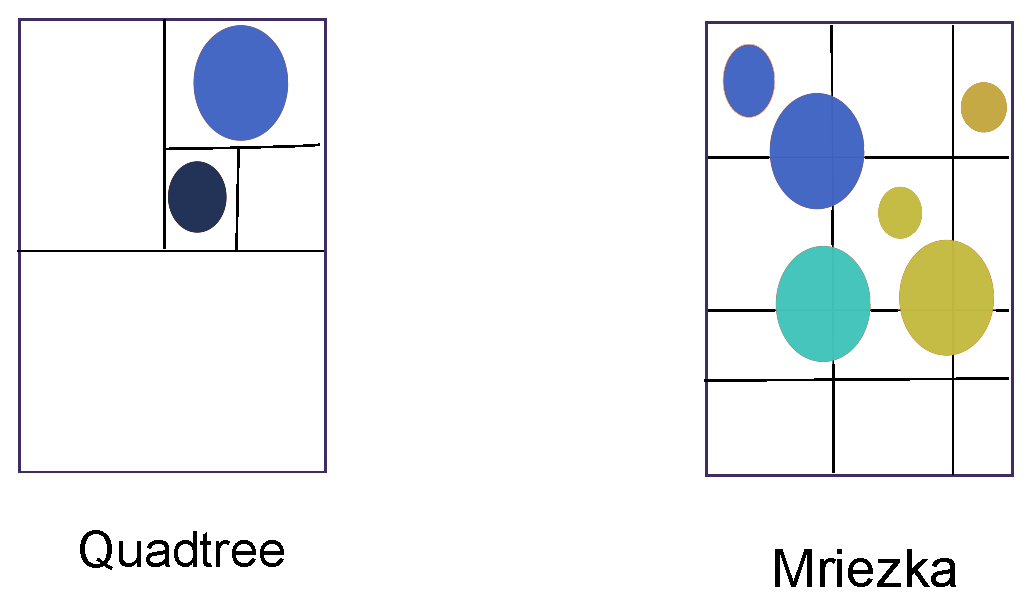
\includegraphics[totalheight=0.2\textheight,width=.5\textwidth]{mriezka}
\caption{Porovnanie quadtree a mriežky}
\label{fig:qtreemriezka}
\end{figure}
Pre lepšiu implementovateľnosť bola zvolená mriežková metóda. \\
Keď máme vyriešený spôsob, akým sa rieši kolízia, je treba určiť, ako na ňu jednotlivé objekty reagujú. Rozhodli sme sa takto:
\begin{description}
\item [Robot vs. strela] Strela ukončí svoj život výbuchom a uštedrí robotovi náležité zranenie. Robotovi sa v tomto okamihu ako dôsledok preruší akákoľvek činnosť, ktorú predtým vyvíjal, napríklad pohyb. To čiastočne zodpovedá nabúraniu programu, ako je tomu u ARES-a. Strela potom už z hroe uvedených príčin nepokračuje. Je však na ďalšom rozširení programu, ako sa strela po zásahu bude chovať. Strela môže zasiahnúť aj toho, kto ju vystrelil. Z toho dôvodu, aby robot nemal tendenciu strieľať všade, ale aby bol prinútenú rozmýšľať, či to neublíži aj jemu. Z toho dôvodu je rychlosť striel vždy vyššia ako rýchlosť robota.% oskontrolovat.
\item [Robot vs. Robot] Roboti nemôžu navzájom interagovať inak ako ublížením a pri kolízií sa teda aplikuje útok na blízko. Tento spôsob zľahčuje písanie algoritmu, nakoľko sa nemusí explicitne deklarovať útok nablízko  (útok na diaľku algoritmus musí explicitne vyjadriť, útok na blizko je automatický ). Útok na blízko bude prevedený iba robotom, ktorý spôsobil kolíziu. %TODO rozviest
\item [Robot vs. stena] Robot sa vzhľadom na funkciu steny, tak, ako bola definovaná, zastaví
\item [Robot vs. 5osuvná stena ] Posuvná stena má schopnosť meniť svoje miesto. Robot ju má možnosť posunúť (musí byť pri nej a pohybovať sa). Stena by sa mala hýbať len s robotom, keďže cieľom je, aby mu sústavne poskytovala úkryt. Stena sa tak pri kontakte s robotom posunie v smere, v akom ide robot, v súlade s fyzikálnymi zákonmi. Ak sa snažia stenu posúvať dvaja roboti a smer ich pohybu je vyjadrený dojrozmernym vektorom, potom sa stena pohybuje v smere vektoroveho súčtu týchto dvoch smerov.
\item[Robot vs. prepadlisko] Robot by na prepadlisko nemal stúpať. Z definície musí byť robot potrestaný, keď vstúpi na toto políčko. Ako najjednoduchší spôsob sa ponúka strata životov a následne zastavenie alebo prejdenie prepadliska za cenu niekoľkonásobnej straty životov. Bol implementovaný druhý spôsob. Pri prejdeni prepadliska aj za cenu toho, že bude robot polomŕtvy, sa pri dostatočnom množsve sa života môže ešte podieľať na simulácii.
\item [Stena vs. strela] Strela sa  bude môcť od obyčajnej steny odrážať. Stena nie je nikdy primárnym cieľom. Preto nemá zmysel, aby strela ukončila svoju dráhu pri narazeni na stenu. Jediný dôsledok by bol, že robot môže strelu vidieť a tým by bola prezradena pozícia strelca. Ak sa strela bude ďalej pohybovať, aj keď iným smerom, bude možné strieľať aj za "rohom", umýselne mýliť protivníka vyslanim strely tak, aby sa odrazila, zaútočiť na robota a pritom nedať robotovi žiadnu informáciu o svojej pozícií, zasiahnuť robota, aj ked sa schovava ( aby neexistovalo nič ako dokonalý úkryt ). Preto bolo rozhodnuté o odrazení strely od steny. 
\item[Stena vs. posuvná stena] Stena z definície bráni pohybu. Teda logicky bráni pohybu aj posuvnej stene a následne robotovi za ňou.
\item[Posuvná stena vs. posuvná stena] Posuvná stena má ako hlavný cieľ poskytknúť úkryt, preto nemá zmysel, aby vyvolala pohyb druhej stenou, keď to robot nečaká. Nič to neprinesie. Na druhej strane je zbytočné komplikovať si implenetáciu tým, že sa špeciálne pre istý ibjekt sa stena zastaví. Preto stenou môže pohnúť každý objekt
\item[Strela vs. posuvná stena] Otázkou je, či by sa mala posuvná stena hýbať aj pri kontakte so strelou. Keďže strela vlastne vykonáva útok robota na diaľku, je možné stenou posunúť a to v smere strely. Strela sa súčastne odrazí. % ono je to vpodstate jedno
\item [Strela vs Strela] \hfill \newline
Strela nijak neprofituje so zrážky s inou strelou, takže sa nič nestane. Bolo by možné síce strelu ďalšou strelou odchýliť, ale to znamená pre robota zložité vypočítavanie, kde je strela, kde strela bude a v akom smere má vystrediť. Výsledkom je vyhnutie sa strele, čo zvládne obyčajný pohyb rýchlejšie. 
\end{description}
